\appendix

\section{Supporting System Data}
\label{sec:appendix_system_data}

\begin{table}[htbp]
\centering
\caption{Agility specifications for representative tasked EO satellites, scaled to a \ang{90} slew.}
\label{tab:agility}
\sisetup{table-format=2.1}
\begin{tabular}{@{}l c c l S@{}}
\toprule
\textbf{Platform} & \textbf{Launch} & \textbf{FoR} & \textbf{Manufacturer spec} & {\textbf{Scaled \ang{90} slew [s]}} \\
\midrule
WorldView-1~\citep{maxar_technologies_worldview-1_nodate} & 2007 & $\pm\ang{45}$ & \SI{2.5}{\degree/\second^2},\ \SI{4.5}{\degree/\second}\ max & 24.7 \\
Pl{\'e}iades 1A/1B~\citep{amram_pleiades_nodate}          & 2011 & $\pm\ang{47}$ & \ang{60} in \SI{25}{\second} (incl.\ settle)                 & 37.5 \\
SPOT-6~\citep{noauthor_spot6_nodate}                      & 2012 & $\pm\ang{45}$ & \ang{30} in \SI{14}{\second}                                 & 42.0 \\
Pl{\'e}iades Neo~\citep{noauthor_pleiades_nodate}         & 2022 & $\pm\ang{47}$ & \ang{60} in \SI{20}{\second}                                 & 30.0 \\
\bottomrule
\end{tabular}
\end{table}

\section{Proofs and Derivations}
\label{sec:appendix_proofs}

\subsection{FoR-Edge Projection}
\label{sec:appendix_fov_projection}

The nadir and rolled horizontal-FoV constraints use the same rectilinear projection of a primary-imager FoR edge.
Let $a=R_E+h$, $\beta=\Theta_v/2$, $\rho_F=\rho(\theta_{\mathrm{FoR}})$, $R_F=\sqrt{R_E^2-\rho_F^2}$, and let $\sigma\in\{-1,+1\}$ index the two FoR edges, with $F$ denoting the fixed FoR-edge slice.
Use the same local frame as \figref{fig:lookahead_geometry}: $x$ is the forward local-horizontal projection from $N$, $\sigma\rho_F$ is the cross-track local-horizontal projection of the FoR edge, and $z(x)$ is the component from $S$ toward Earth along the nadir line $SN$.
For a point on either FoR edge, that nadir-axis depth and the forward limb coordinate are
\begin{equation}
z(x)=a-\sqrt{R_F^2-x^2},
\qquad
x_{\mathrm{limb}}=\sqrt{R_E^2\left(1-\left[\frac{R_E}{a}\right]^2\right)-\rho_F^2}.
\label{eq:rolled_body_ray}
\end{equation}
For body roll $\varphi$, the detector-plane horizontal offset, vertical offset, and boresight depth are
\begin{equation}
\begin{aligned}
\delta_\sigma(x;\varphi)
&=\sigma\rho_F\cos\varphi-z(x)\sin\varphi,\\
\eta_\sigma(x;\varphi)
&=x\cos\beta-\sin\beta\left[z(x)\cos\varphi+\sigma\rho_F\sin\varphi\right],\\
d_\sigma(x;\varphi)
&=x\sin\beta+\cos\beta\left[z(x)\cos\varphi+\sigma\rho_F\sin\varphi\right].
\end{aligned}
\label{eq:rolled_body_depth_offset}
\end{equation}
The rectangular-detector condition is
\begin{equation}
\mathcal{D}_\sigma(\varphi) =
\left\{x\in[0,x_{\mathrm{limb}}]\;:\;
\left|\eta_\sigma(x;\varphi)\right|\leq d_\sigma(x;\varphi)\tan\beta,\;
d_\sigma(x;\varphi)>0\right\},
\label{eq:rolled_vertical_band}
\end{equation}
and the horizontal look angle is
\begin{equation}
\lambda_\sigma(x;\varphi)=
\operatorname{atan2}\!\left(\delta_\sigma(x;\varphi),d_\sigma(x;\varphi)\right).
\label{eq:rolled_horizontal_angle}
\end{equation}
The key point is that this is a flat focal-plane condition; replacing it with a viewing-sphere latitude bound describes a different detector.

\subsection{Nadir-FoR Limiting Point}
\label{sec:appendix_nadir_fov}

The nadir-FoR requirement in~\eqref{eq:horizontal_fov_requirement} is the $\varphi=0$ specialization of the FoR-edge projection.
The limiting point lies on a FoR edge with cross-track coordinate $\rho_F$.
With $a=R_E+h$ and $\beta=\Theta_v/2$, the upper detector edge is the rectilinear condition
\begin{equation}
\frac{x\cos\beta-z\sin\beta}
{x\sin\beta+z\cos\beta}
=\tan\beta
\quad\Longleftrightarrow\quad
\frac{x}{z}=\tan\Theta_v.
\label{eq:nadir_upper_edge_condition}
\end{equation}
Combining~\eqref{eq:nadir_upper_edge_condition} with the spherical height relation
$z=a-\sqrt{R_F^2-x^2}$ gives the upper-edge contact
\begin{equation}
x_{\mathrm{edge}} =
\sin\Theta_v
\left[
a\cos\Theta_v
-\sqrt{R_F^2-a^2\sin^2\Theta_v}
\right],
\label{eq:nadir_upper_edge_contact}
\end{equation}
provided the square-root term is real and the upper edge intersects Earth before the limb.
Otherwise the limiting point is the forward limb point on the same FoR edge,
\begin{equation}
x_{\mathrm{limb}} =
\sqrt{
R_E^2\left(1-\left[\frac{R_E}{a}\right]^2\right)-\rho_F^2
}.
\label{eq:nadir_horizon_cap}
\end{equation}
The transition occurs when the upper detector edge first reaches the limb,
\begin{equation}
\Theta_v
=
\arcsin\!\left(\frac{R_F}{a}\right).
\label{eq:nadir_limb_transition}
\end{equation}

\subsection{Rolled-Body FoR Candidate Equations}
\label{sec:appendix_rolled_fov}

The rolled-body requirement in~\eqref{eq:rolled_body_horizontal_requirement} uses the same FoR-edge projection with $\varphi=\theta_{\mathrm{FoR}}$.
Under this roll convention, the same-side FoR point is pinned to the lower detector center and the opposite FoR edge sets the horizontal width.
The upper-edge contact in~\eqref{eq:rolled_opposite_contact} is the admissible root, for $\sigma=-1$, of
\begin{equation}
\eta_\sigma(x;\varphi)=d_\sigma(x;\varphi)\tan\beta.
\label{eq:rolled_vertical_boundary}
\end{equation}
Equivalently, with $z(x)=a-\sqrt{R_F^2-x^2}$,
\begin{equation}
x=\tan(2\beta)
\left[z(x)\cos\varphi+\sigma\rho_F\sin\varphi\right].
\label{eq:rolled_upper_edge_contact}
\end{equation}
With the same shorthand used in the main text,
$Q=\cot(2\beta)$ and $K_\sigma=a\cos\varphi+\sigma\rho_F\sin\varphi$.
Substituting $z(x)=a-\sqrt{R_F^2-x^2}$ into~\eqref{eq:rolled_upper_edge_contact} gives
$Qx=K_\sigma-\cos\varphi\sqrt{R_F^2-x^2}$, so the candidate roots satisfy
\begin{equation}
\left(\cos^2\varphi+Q^2\right)x^2
-2K_\sigma Qx
+K_\sigma^2-\cos^2\varphi\,R_F^2=0.
\label{eq:rolled_upper_edge_quadratic}
\end{equation}
The closed form in~\eqref{eq:rolled_upper_contact_closed_form} follows from this quadratic.
Roots are retained only if they satisfy the unsquared relation
$Qx=K_\sigma-\cos\varphi\sqrt{R_F^2-x^2}$ and the front-facing vertical-band constraint $x\in\mathcal{D}_\sigma(\varphi)$.
For the opposite-edge engineering expression, $x_{\mathrm{upper}}$ is the retained $\sigma=-1$ root that minimizes $\left|\lambda_-(x;\varphi)\right|$.

The fully general implementation evaluates $\left|\lambda_\sigma(x;\varphi)\right|$ on a finite candidate set for both $\sigma\in\{-1,+1\}$ and keeps points satisfying $x\in\mathcal{D}_\sigma(\varphi)$.
This set consists of the interval endpoints $x=0$ and $x=x_{\mathrm{limb}}$, detector-edge contacts from~\eqref{eq:rolled_vertical_boundary}, and interior stationary contacts of
$\lambda_\sigma(x;\varphi)=\operatorname{atan2}(\delta_\sigma(x;\varphi),d_\sigma(x;\varphi))$.
Since
\begin{equation}
\frac{d\lambda_\sigma}{dx}=0
\quad\Longleftrightarrow\quad
d_\sigma(x;\varphi)\delta_\sigma'(x;\varphi)-\delta_\sigma(x;\varphi)d_\sigma'(x;\varphi)=0,
\label{eq:rolled_stationary_condition}
\end{equation}
the stationarity condition can be written compactly as
\begin{equation}
p_\sigma x+q_\sigma\sqrt{R_F^2-x^2}+r=0,
\label{eq:rolled_stationary_compact}
\end{equation}
where
\begin{equation}
p_\sigma=\sigma\rho_F\cos\beta,\qquad
q_\sigma=\sin\beta\left[\sigma\rho_F\cos\varphi-a\sin\varphi\right],
\qquad
r=R_F^2\sin\beta\sin\varphi.
\end{equation}
Squaring~\eqref{eq:rolled_stationary_compact} gives the quadratic candidate equation
\begin{equation}
(p_\sigma^2+q_\sigma^2)x^2
 +2p_\sigma r\,x
 + r^2-q_\sigma^2R_F^2 = 0.
\label{eq:rolled_stationary_quadratic}
\end{equation}
Because squaring can introduce extraneous roots, stationary candidates from~\eqref{eq:rolled_stationary_quadratic} are kept only if they also satisfy the unsquared condition~\eqref{eq:rolled_stationary_compact}.
If no candidate remains for either one of the two FoR edges, the rolled body-fixed configuration is infeasible for that $(\Theta_v,\theta_{\mathrm{FoR}})$ pair.

\subsection{Two-Boundary Renewal Estimator}
\label{sec:appendix_renewal}

This appendix derives the support-aware two-boundary probability in~\eqref{eq:chain_prob} and records the residual bias source for the finite-window estimator used in \secref{sec:heuristic}.
The main text gives the estimator and the break-even surrogate; the derivation below shows why the incomplete-gamma term is the anchored packing probability.

\subsection{Derivation of the Two-Boundary Chain Probability}

Place the two schedule anchors at positions $0$ and $L$, and let the detector reveal clear candidates only on the support interval $[\ell,r]\subseteq[0,L]$.
Consider $k$ internal chain points
\begin{equation}
\ell \leq t_1 < t_2 < \dots < t_k \leq r.
\end{equation}
The anchor spacing constraints are $t_1 \geq g$, $t_{i+1}-t_i \geq g$ for $i=1,\dots,k{-}1$, and $L-t_k \geq g$.
The boundary constraints only remove support that lies too close to the anchors, so define
\begin{equation}
c_L=\max(0,g-\ell),\qquad
c_R=\max(0,g-(L-r)),\qquad
U=(r-\ell)-c_L-c_R.
\end{equation}
After trimming these boundary clearances, the first accepted point can occur at the start of the usable interval, while each additional internal point requires one deterministic clearance $g$ plus one exponential wait.
Under Poissonization~\cite{jacquet_analytical_1998, feller_probability_1948}, the total time needed to place $k$ internal points inside usable support is
\begin{equation}
S_k = (k{-}1)g + \underbrace{\sum_{i=1}^{k} X_i}_{Y_k},
\end{equation}
where $Y_k \sim \Gamma(k, \lambda)$ as a sum of i.i.d.\ exponentials~\cite{feller_introduction_1991}.
Equivalently, the $k$ internal points correspond to $k$ Poisson arrivals falling in the residual interval of length $U-(k{-}1)g$.
By the Poisson--Gamma duality $P(\mathrm{Pois}(\mu) \geq k) = \gamma(k, \mu)/\Gamma(k)$ with $\mu = \lambda\bigl(U-(k{-}1)g\bigr)$, giving~\eqref{eq:chain_prob}.
The shape parameter is $k$ because fitting $k$ internal arrivals requires $k$ exponential waits; the anchor clearances and the $k{-}1$ internal clearances are deterministic.
This corresponds to the \emph{non-paralyzable} (Type~I) counter convention with both ends anchored~\cite{pyke_renewal_1958}.
When $[\ell,r]=[0,L]$, $U=L-2g$ and the residual interval becomes $L-(k{+}1)g$, recovering the standard full-support two-boundary form.

\subsection{Proof of Proposition~\ref{prop:omniscience} (Instant-Slew Omniscience)}

With zero slew time, a lookahead can be inserted immediately before each candidate access at no opportunity cost.
Because onboard observations are assumed noise-free, every cloud state $X_i$ is revealed before the corresponding imaging decision is made.
The scheduler can therefore solve~\eqref{eq:scheduling} with realized utilities $u_i = c_i \cdot X_i$ in place of expected utilities, recovering the omniscient optimum. \qed

\subsection{Proof of Proposition~\ref{prop:timing} (Optimal Lookahead Timing)}

Decompose
$\widehat{\Delta J}(t)/\bar{c}
= E[K;\, \lambda_c(t),\, W(t),\, \ell(t),\, r(t),\, L_{\mathrm{anc}},\, g]
- p\, N_{\mathrm{sched}}(t)
- \hat{J}^-(t)/\bar{c}$,
where $E[K;\cdot]$ is the support-aware two-boundary chain-length estimator from~\eqref{eq:chain_expectation} applied to the clipped detector support $[\ell(t),r(t)]$ inside the fixed anchor interval.
Both $N_{\mathrm{obs}}(t)$ and the support end $r(t)$ are non-decreasing step/continuous functions of $t$: they grow when visible accesses or newly reachable detector support enter the actionable window $[t_{\mathrm{next}},\, t+t_{\mathrm{horizon}}]$.
Between access entries, the chain term is smoothly non-decreasing in the clipped support at fixed $N_{\mathrm{obs}}$.
If the baseline is charged only once per fixed schedule gap, as in the implementation, this monotonicity is direct; if scheduled tasks are charged as they enter the local window, $N_{\mathrm{sched}}(t)$ is a non-decreasing step function and the following bounded-jump argument applies.
At a scheduled-access entry, $p\, N_{\mathrm{sched}}$ jumps up by $p$ while the chain term jumps up by the marginal contribution of one additional candidate (bounded by $p$ since each new candidate is independently clear with probability $p$); the net jump in $\widehat{\Delta J}$ is therefore bounded below by $-p\bar{c}$.
Hence $\widehat{\Delta J}$ is piecewise-smoothly non-decreasing with bounded downward steps of size at most $p\bar{c}$ while $\hat{J}^-=0$.

For $t \leq t^\star(\alpha)$, the maneuver terminates no later than $t_{\mathrm{next}}$, so $\hat{J}^- = 0$ and the net advantage is the finite-window chain value minus the local baseline burden.
For $t > t^\star(\alpha)$, $\hat{J}^-$ steps up by $p\bar{c}$ for each scheduled task whose imaging time falls in the maneuver interval $[t,\, t+t_{\mathrm{man}}(\alpha)]$, which equals or exceeds the concurrent marginal gain of $\hat{J}^+$ so the net advantage is non-increasing past $t^\star(\alpha)$.
Therefore $t^\star(\alpha)$ maximizes $\widehat{\Delta J}$ up to at most one bounded perturbation of size $p\bar{c}$, with equality when no scheduled access enters the observation window within a small left-neighborhood of $t^\star(\alpha)$.
\qed

\section{Bias Analysis Details}
\label{sec:appendix_bias}

The two-boundary form in~\eqref{eq:chain_prob} already absorbs the dominant bias source present in a naive one-anchor renewal estimate: the usable support $U$ explicitly removes only the detector support that violates the left or right anchor clearance, rather than over-counting free space near $0$ and $L$.
The remaining bias is small and of a single sign.

\paragraph{Poissonization variance (residual negative bias).}
Replacing $N$ fixed points with $\mathrm{Poisson}(N)$ introduces count variance.
Since the chain length $f(n)$ is concave in the number of points (diminishing returns), Jensen's inequality gives $\mathbb{E}[f(\mathrm{Poisson}(N))] \leq f(N)$, producing a small negative bias.
A standard de-Poissonization correction~\cite{jacquet_analytical_1998} can be applied but achieves near-zero mean bias at the cost of increased variance from numerical sensitivity, offering no net RMSE improvement.
We therefore use the uncorrected~\eqref{eq:chain_prob} when reporting the finite-window score.

\section{IID Scheduling Numerical Summary}
\label{sec:appendix_iid_scheduling_summary}

\begin{table}[H]
    \centering
    \begin{tabular}{@{}rrlccc@{}}
\toprule
FoV [deg] & $t_{\mathrm{slew}}$ [s] & Policy & Gap closed [\%] & Lookaheads/access & Lookaheads/trial \\
\midrule
45 & 25 & greedy & $50.4 \pm 5.0$ & $0.321 \pm 0.032$ & $176.2 \pm 89.2$ \\
45 & 25 & break-even & $75.1 \pm 5.7$ & $0.149 \pm 0.012$ & $79.9 \pm 37.2$ \\
45 & 25 & two-anchor & $75.1 \pm 6.0$ & $0.154 \pm 0.015$ & $83.6 \pm 40.9$ \\
\addlinespace[0.2em]
45 & 35 & greedy & $36.6 \pm 6.6$ & $0.288 \pm 0.022$ & $138.4 \pm 67.6$ \\
45 & 35 & break-even & $66.6 \pm 5.3$ & $0.143 \pm 0.010$ & $65.9 \pm 25.6$ \\
45 & 35 & two-anchor & $67.1 \pm 5.3$ & $0.152 \pm 0.008$ & $71.3 \pm 30.9$ \\
\addlinespace[0.2em]
45 & 45 & greedy & $25.0 \pm 6.6$ & $0.282 \pm 0.020$ & $118.2 \pm 55.3$ \\
45 & 45 & break-even & $59.6 \pm 5.0$ & $0.144 \pm 0.019$ & $57.8 \pm 22.7$ \\
45 & 45 & two-anchor & $61.0 \pm 5.3$ & $0.160 \pm 0.018$ & $64.2 \pm 24.1$ \\
\midrule
60 & 25 & greedy & $69.5 \pm 4.5$ & $0.342 \pm 0.040$ & $188.7 \pm 98.0$ \\
60 & 25 & break-even & $86.5 \pm 5.6$ & $0.179 \pm 0.014$ & $96.0 \pm 44.6$ \\
60 & 25 & two-anchor & $86.7 \pm 5.5$ & $0.179 \pm 0.013$ & $96.1 \pm 44.7$ \\
\addlinespace[0.2em]
60 & 35 & greedy & $56.3 \pm 6.4$ & $0.315 \pm 0.029$ & $152.3 \pm 76.1$ \\
60 & 35 & break-even & $87.2 \pm 3.6$ & $0.189 \pm 0.012$ & $89.8 \pm 40.8$ \\
60 & 35 & two-anchor & $87.6 \pm 3.8$ & $0.190 \pm 0.013$ & $90.3 \pm 41.8$ \\
\addlinespace[0.2em]
60 & 45 & greedy & $45.7 \pm 5.9$ & $0.309 \pm 0.030$ & $130.3 \pm 62.8$ \\
60 & 45 & break-even & $84.1 \pm 6.2$ & $0.200 \pm 0.020$ & $82.1 \pm 35.2$ \\
60 & 45 & two-anchor & $85.3 \pm 6.7$ & $0.208 \pm 0.021$ & $85.9 \pm 37.8$ \\
\bottomrule
\end{tabular}

    \caption{Numerical summary for the paired iid scheduling trials in \figref{fig:iid_scheduling_tradeoff}. Entries report mean $\pm$ one standard deviation across trials.}
    \label{tab:iid_scheduling_summary}
\end{table}
\FloatBarrier

\section{BCM Scheduling Numerical Summary}
\label{sec:appendix_bcm_scheduling_summary}

\begin{table}[H]
    \centering
    \begin{tabular}{@{}rrlccc@{}}
\toprule
FoV [deg] & $t_{\mathrm{slew}}$ [s] & Policy & Gap closed [\%] & Lookaheads/access & Lookaheads/trial \\
\midrule
45 & 25 & greedy & $39.6 \pm 12.5$ & $0.259 \pm 0.017$ & $66.7 \pm 7.9$ \\
45 & 25 & break-even & $70.0 \pm 5.7$ & $0.130 \pm 0.006$ & $33.6 \pm 3.8$ \\
45 & 25 & two-anchor & $69.8 \pm 6.4$ & $0.130 \pm 0.006$ & $33.5 \pm 3.8$ \\
\addlinespace[0.2em]
45 & 35 & greedy & $19.9 \pm 12.0$ & $0.247 \pm 0.015$ & $56.5 \pm 7.1$ \\
45 & 35 & break-even & $59.0 \pm 10.5$ & $0.141 \pm 0.008$ & $32.4 \pm 4.0$ \\
45 & 35 & two-anchor & $62.7 \pm 8.0$ & $0.151 \pm 0.008$ & $34.8 \pm 4.7$ \\
\addlinespace[0.2em]
45 & 45 & greedy & $4.5 \pm 12.3$ & $0.253 \pm 0.013$ & $51.2 \pm 5.0$ \\
45 & 45 & break-even & $57.3 \pm 9.5$ & $0.171 \pm 0.014$ & $34.5 \pm 3.4$ \\
45 & 45 & two-anchor & $61.4 \pm 7.0$ & $0.179 \pm 0.010$ & $36.2 \pm 3.5$ \\
\midrule
60 & 25 & greedy & $67.8 \pm 6.3$ & $0.274 \pm 0.020$ & $70.7 \pm 10.5$ \\
60 & 25 & break-even & $77.8 \pm 5.2$ & $0.158 \pm 0.008$ & $40.8 \pm 4.4$ \\
60 & 25 & two-anchor & $78.9 \pm 4.6$ & $0.158 \pm 0.008$ & $40.6 \pm 4.4$ \\
\addlinespace[0.2em]
60 & 35 & greedy & $49.2 \pm 11.5$ & $0.277 \pm 0.021$ & $63.3 \pm 7.4$ \\
60 & 35 & break-even & $76.4 \pm 5.5$ & $0.174 \pm 0.014$ & $39.6 \pm 3.3$ \\
60 & 35 & two-anchor & $76.6 \pm 5.3$ & $0.173 \pm 0.014$ & $39.4 \pm 3.3$ \\
\addlinespace[0.2em]
60 & 45 & greedy & $39.5 \pm 10.9$ & $0.276 \pm 0.026$ & $56.0 \pm 7.1$ \\
60 & 45 & break-even & $80.1 \pm 7.8$ & $0.196 \pm 0.015$ & $39.6 \pm 3.8$ \\
60 & 45 & two-anchor & $81.3 \pm 6.6$ & $0.198 \pm 0.014$ & $40.0 \pm 3.5$ \\
\bottomrule
\end{tabular}

    \caption{Numerical summary for the paired BCM scheduling trials in \figref{fig:bcm_scheduling_tradeoff}. Entries report mean $\pm$ one standard deviation across trials.}
    \label{tab:bcm_scheduling_summary}
\end{table}
\FloatBarrier

\section{Two-Boundary Chain Probability Validation}
\label{sec:appendix_chain_probability}

\figref{fig:chain_probability_validation} validates the probability term in~\eqref{eq:chain_prob} directly.
For fixed interval length $L=\num{10}$ and expected candidate count $N=\num{20}$, the plot sweeps the required spacing $g$ and compares the analytic probability $G(k;\lambda,L,g)$ with Monte Carlo estimates of whether at least $k$ internal points can be packed between the two anchors.
The agreement shows that the incomplete-gamma expression captures the anchored chain feasibility event itself; Experiment~1 then applies the same chain model after Bernoulli cloud thinning and subtracts the local baseline burden.

\begin{figure}[H]
    \centering
    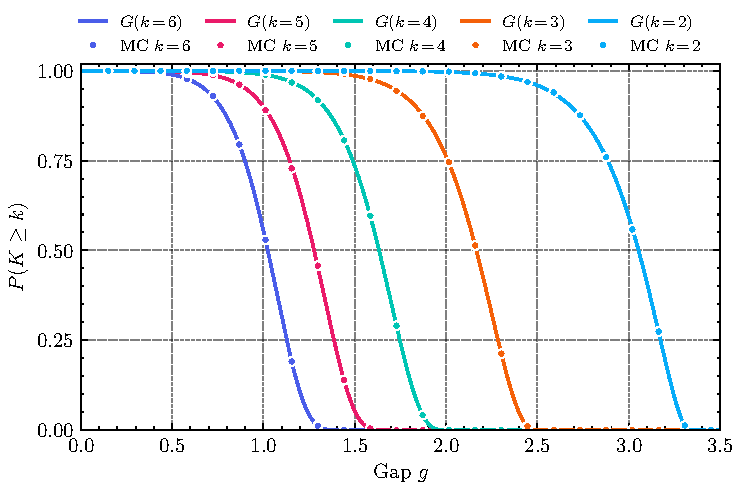
\includegraphics[width=0.78\linewidth]{figures/chain_probability.pdf}
    \caption{Validation of the two-boundary chain probability in~\eqref{eq:chain_prob}. Solid curves show the analytic expression $G(k;\lambda,L,g)$; markers show Monte Carlo estimates for the same anchored packing event.}
    \label{fig:chain_probability_validation}
\end{figure}
